\chapter{State of the art analysis}\label{chap:chap3}

In this chapter it is presented the related work. It are introduced  some electronic assessment tools that are currently being used in the market and others made for teaching purposes.

\section{CMMI assessment checklist}

CMMI assessment checklist \citep{capabilityassess} appears as an online solution to make a lightweight assessment tool and is a free online assessment tool that make possible get and track an organization capability across eight key business functions based in a group of 31 questions.


\textbf{Assessment items}

In this tool, each assessment item has a statement about a particular capability or several capabilities and a scale that allows to indicate the level of agreement with the statement, based on the organization performance. An example is shown in Figure \ref{fig:cmmi_question}.

\begin{figure}[h]
	\begin{center}
		\leavevmode
		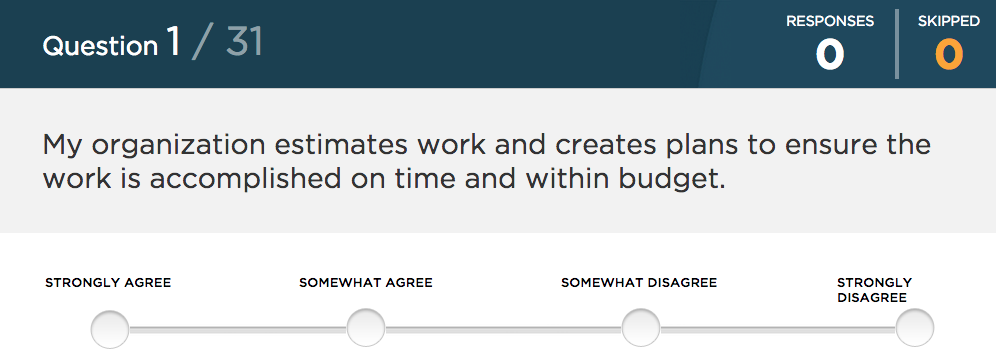
\includegraphics[width=0.9\textwidth]{cmmi_question}
		\caption{Assessment item question}
		\label{fig:cmmi_question}
	\end{center}
\end{figure}

The scale included in the assessment item also includes a descriptive information about the organization performance at both ends of the scale, visible on the example given in Figure \ref{fig:assesment_answer}.

\begin{figure}[h]
	\begin{center}
		\leavevmode
		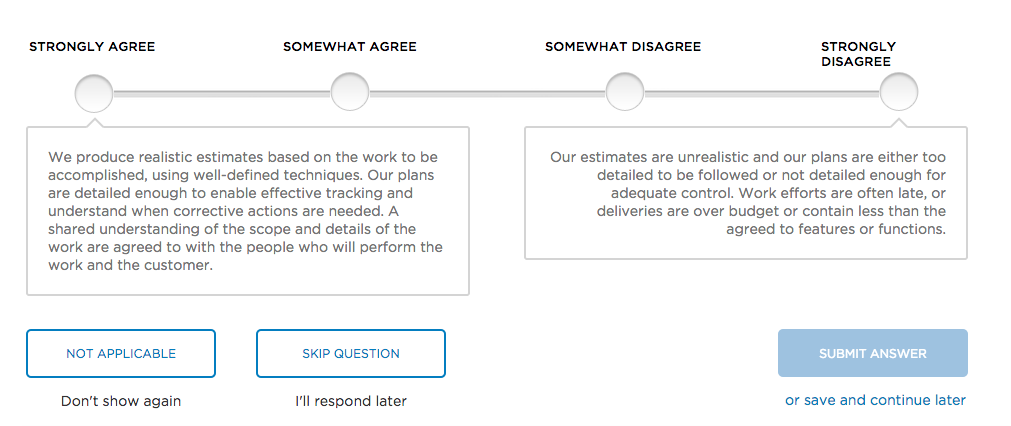
\includegraphics[width=1\textwidth]{respostascmmiassessment}
		\caption{Assessment item scale}
		\label{fig:assesment_answer}
	\end{center}
\end{figure}

These descriptions are given to the user with the intention of helping the most accurate positioning of the organization on the scale.

The organization term in the assessment tool is defined by the user for purposes of  self-assessment. The evaluated scope is also defined by the user and can be the company, organizational unit, division, directorate, department or work group.

It's possible to skip a question in the list of items and comeback later to answer and there is an option named Not Applicable to exclude the question from the results. This answer only should be chosen if:
\begin{itemize}
	\item The actual question is related to an area outside of the organization scope.
	\item It's valid for the organization but the  performance of the activity is not known.
	\item The user that is performing the assessment has insufficient expertise in the subject to understand the intent of the question.
\end{itemize}

The answers are editable before the submission of the assessment in a screen for a final review. It is possible to save the current state and progress at any time and resume it later. It is only possible to submit and get an assessment if all questions are answered.

After answering all questions provided as requirement the survey is submitted and will be shown a high level snapshot of the organization  current capability states and will be included in each item some suggestions for developing the next steps as seen in Figure \ref{fig:assesment_result}.

The goal of this research work is to fully automate the assessment for as many practices as possible. As will be explained in Section \ref{sec:question}, we take advantage of some of the questions in this tool to help in the assessment of the remaining practices.

\newpage 

\begin{figure}[h]
	\begin{center}
		\leavevmode
		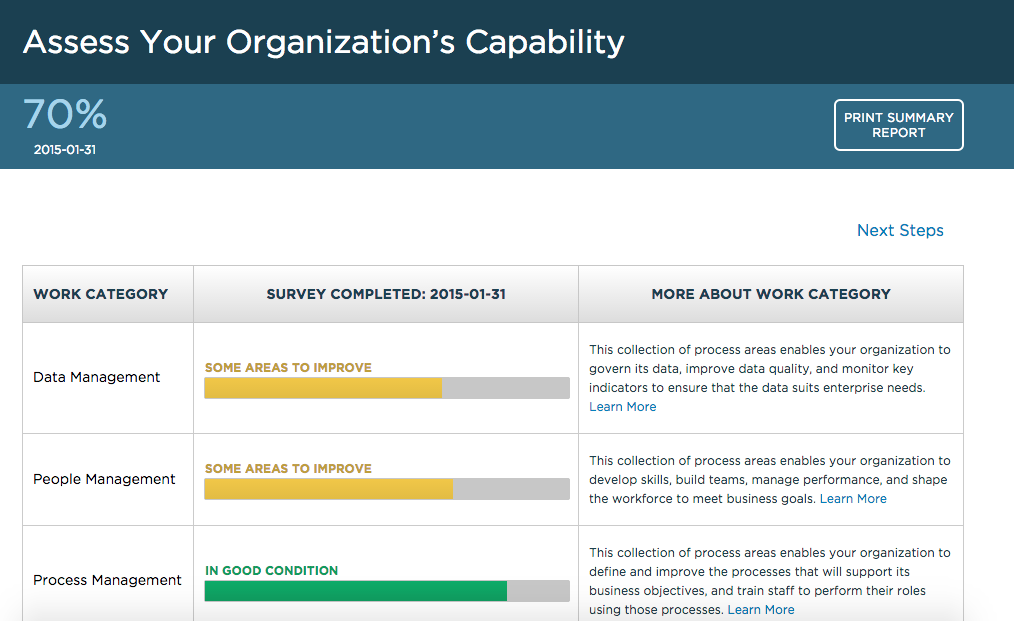
\includegraphics[width=0.96\textwidth]{resultcmmiassessment}
		\caption{Example of a result an assessment}
		\label{fig:assesment_result}
	\end{center}
\end{figure}


\section{PSP checker}

The Personal Software Process (PSP) \citep{humphrey2005psp} is a process framework with the objective of guide developers to define their own processes, track and plan their work and manage the quality of the produced products.

PSP checker \citep{Pinto2010} is a tool developed at FEUP that has the main objective of helping teachers to evaluate the assignments submitted by PSP students  and help them to achieve better results and understand PSP.

The PSP checker was only made and planned for teachers as a support for evaluation and feedback. It is suitable for students too depending on the type of teaching, that way they can improve their work. A short period of time is required to use this tool and is currently available only as a desktop application.


This desktop application has as main functionalities:
\begin{itemize}
	\item Automatic verification of checklists
	\subitem Each checklist item has different types of verification and as output; if an item in the checklist is completely satisfied, it is shown the line in green, otherwise the line is highlighted in red or given a special message on the screen.
	\item Custom processes
	\subitem The user, when starting the program, can choose which items of the PSP process to associate with this evaluation.
	\item Remote data importation
	\item Illustrative charts
	\subitem Charts that facilitate the perception of whats is wrong and well done to understand which points can be improved.
	\item Automation of support messages (use of knowledge acquired by specialists)
	\subitem Messages provided by specialist to understand the errors in a more complex level.
	\item Information Import/Export (Figure \ref{fig:PSPdataimport})
	\item Modularity and scalability
\end{itemize}

\begin{figure}[h]
	\begin{center}
		\leavevmode
		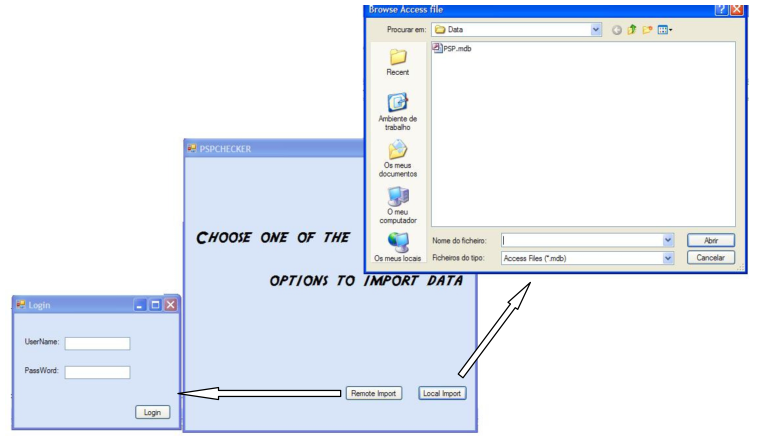
\includegraphics[width=0.63\textwidth]{PSPdataimport}
		\caption{Example of a data import for PSPChecker}
		\label{fig:PSPdataimport}
	\end{center}
\end{figure}

\begin{figure}[h]
	\begin{center}
		\leavevmode
		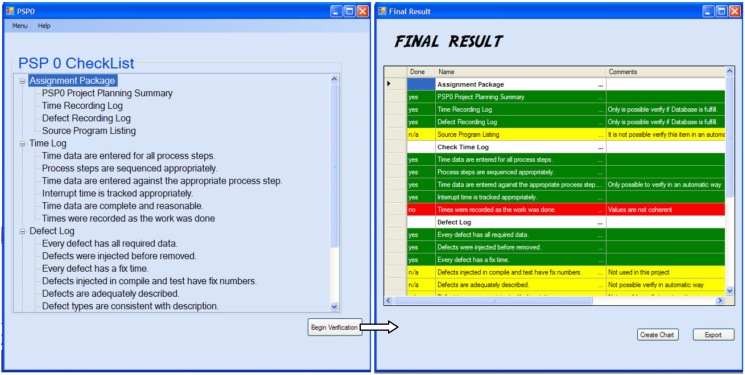
\includegraphics[width=0.8\textwidth]{PSPresult}
		\caption{Final results of PSPChecker}
		\label{fig:PSPresults}
	\end{center}
\end{figure}

In Figure \ref{fig:PSPresults} it are represented two of the last screens of PSPChecker. It is shown on the left hand side the checklist imported or chosen and on the right side the final screen, where we can generate charts and export the data. 
Items successfully checked are colored in green. Items not satisfied are colored in red. Items that could not be evaluated automatically are colored in yellow.

This method of evaluation is used to make a similar approach to CMMI instead of PSP.

\section{Appraisal assistant}

The Software Quality Institute of the Griffith University 	\citep{SoftwareQuality2015} developed the Appraisal Assistant tool. The Appraisal Assistant \citep{Appraisal2015} is a software application that supports the appraisal or assessment of process capability or organization maturity.

This tool follows consistent approaches with the requirements of ISO/IEC 15504 \citep{ISOIEC} and it's distinguished from other tools by taking an evidence-driven approach to the recording of evidences generated in an assessment.

SQI personnels have performed SCAMPI A and B appraisals and SPICE assessments with the help of Appraisal Assistant and have been it using since the first beta release. The Beta release was used to examine relationships between ISO 15504-2 and SCAMPI appraisals

\begin{figure}[h]
	\begin{center}
		\leavevmode
		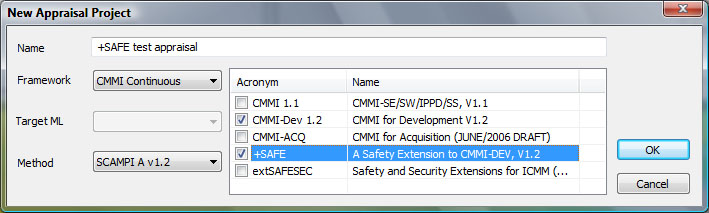
\includegraphics[width=0.8\textwidth]{newprojectsappraisal}
		\caption{Appraisal Assistant New Project Screen}
		\label{fig:newprojectsappraisal}
	\end{center}
\end{figure}

The Appraisal Assistant provides several functionalities and benefits:
\begin{itemize}
	\item Support for multiple process models such as: ISO/IEC 15504-5, ISO/IEC 15504-6 (FDIS) \citep{rout2003iso}, Automotive SPICE, CMMI®-DEV v.1.2, +SAFE, and CMMI® SE/SW/IPPD/SS V 1.1 \citep{team2002capability};
	\item User defined appraisal models;
	\item Multiple methods for performing an appraisal / assessment;
	\item User defined assessment methods;
	\begin{figure}[h]
		\begin{center}
			\leavevmode
			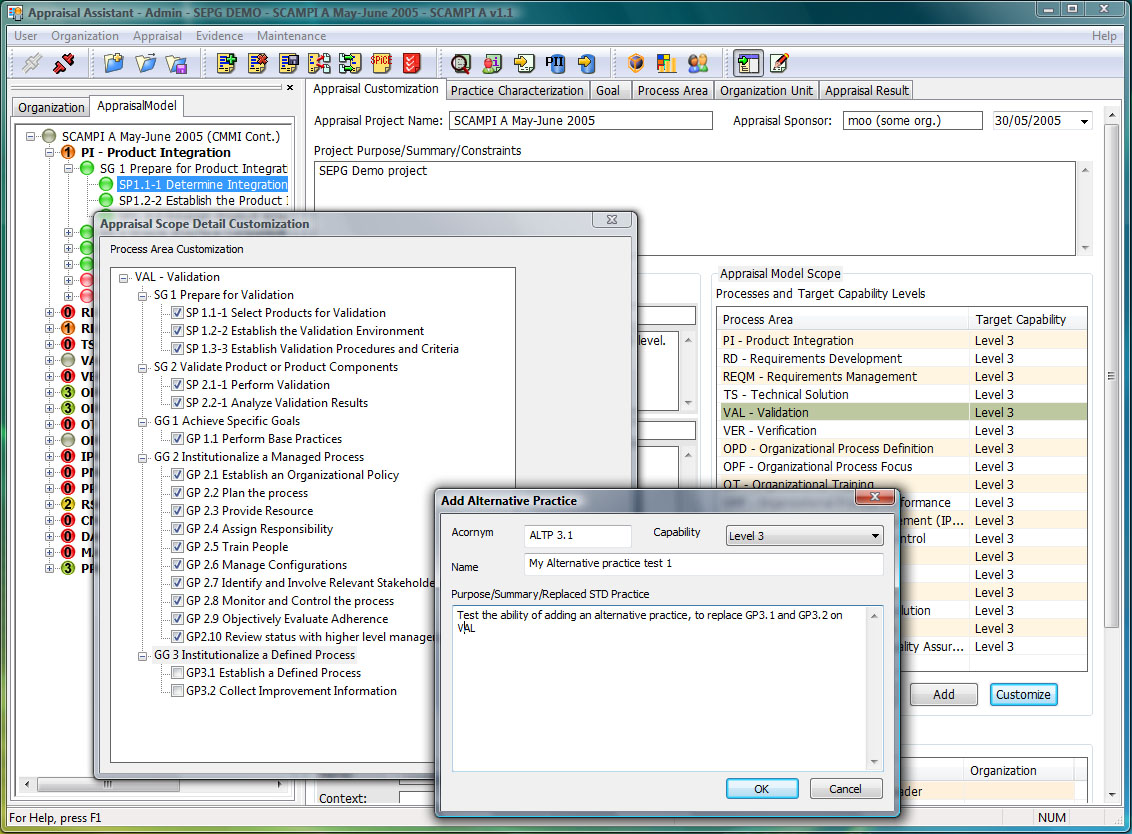
\includegraphics[width=0.6\textwidth]{cmmi_plan}
			\caption{Appraisal Scope Customization}
			\label{fig:cmmi_plan}
		\end{center}
	\end{figure}
	\item Conversion of results between frameworks;
	\item Split and consolidate evidence capture activities;
	\item Generate automatically reports such as Appraisal Disclosure Statement, PIID, Assessment Record, Appraisal / Assessment Findings, Strength / Weakness summaries, Rating Profiles, and workload summaries;
	\item Model coverage and automatic reporting by collected evidence.
\end{itemize}


\begin{figure}[h]
	\begin{center}
		\leavevmode
		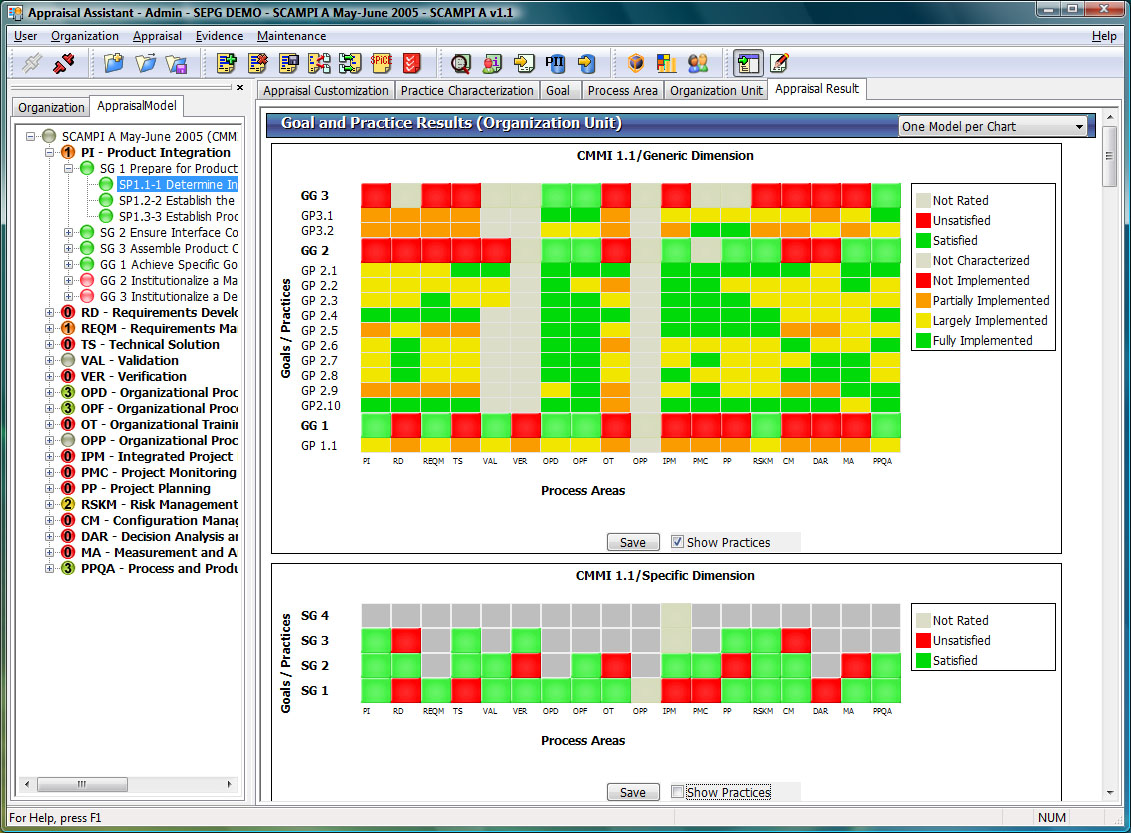
\includegraphics[width=0.6\textwidth]{cmmi_result}
		\caption{Appraisal Assistant Results}
		\label{fig:cmmi_result}
	\end{center}
\end{figure}

In Figure \ref{fig:cmmi_result} it is shown an example of an appraisal result and the output of the tool after labeling all the process areas.

We take advantage of the way results are presented on this tool, regarding CMMI practices organized by their areas, goals and practices.
\newpage


\section{ITMark appraisal tool}

ITmark \citep{ITMARK} is a certification scheme designed specifically for SMEs that combines various improvement models streamlined into only one scheme.

This certification is developed by leading appraisal providers across technical and business related disciplines, gathered in an International Consortium of Centers of Excellence dedicated to support Software Intensive Organizations throughout the world.

This certification assesses and certifies the processes in small organization in three different areas:
\begin{itemize}
	\item Business Management
	\item Software, Systems and Services Engineering
	\item Security Management
\end{itemize}

It provides a group of analysis tools that help a company enhance its business, information security management and software development processes. A company can have additional recognition for their level of capability through ITMark certification.

ITMark will provide organizations:
\begin{itemize}
	\item Process improvement of product development and services
	\item Improvement of other critical processes of the organization: business and security
	\item Low cost and quick implementation of the improvements
	\item Philosophy of quality
	\item Internationally recognized
\end{itemize}

The ITMark Appraisal tool \citep{ITMARKASSESSMENT} fully supports this process.


When an assessment is created in the interface we can access the three areas and see all the specific questions that we need to answer in order to get the results in Figure \ref{fig:itmark_question}, we can see in the top the three areas and an example of a question with the possible answers that are "yes", "no" or "not applicable".

\begin{figure}[H]
	\begin{center}
		\leavevmode
		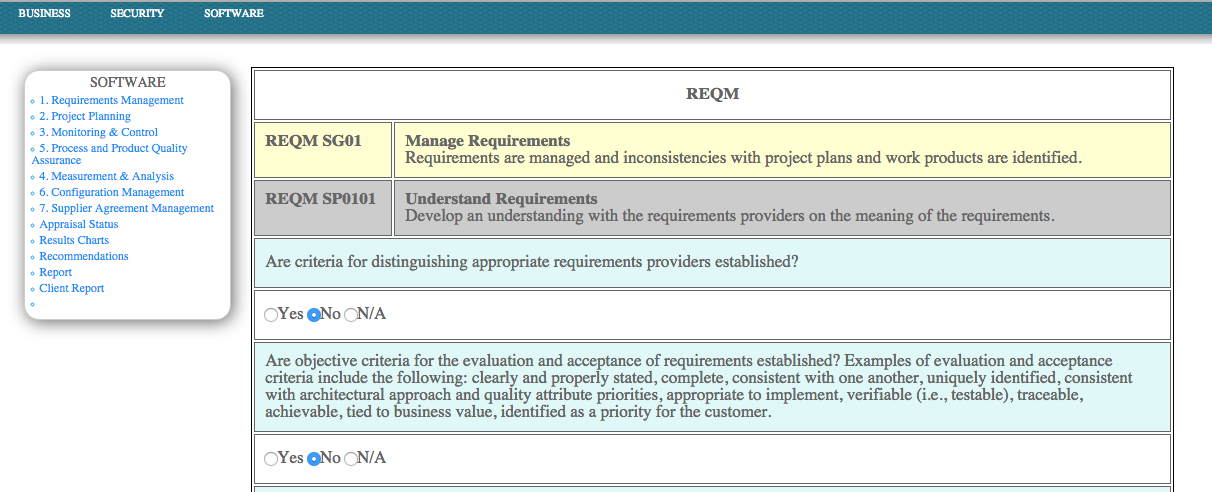
\includegraphics[width=1\textwidth]{question_example_itmark}
		\caption{ITMark Appraisal tool question example}
		\label{fig:itmark_question}
	\end{center}
\end{figure}

After answering all the questions this tool will provide us graphs and some charts with the assessment results. We can see an example of those graphs in Figure \ref{fig:itmark_result1}

\begin{figure}[H]
	\begin{center}
		\leavevmode
		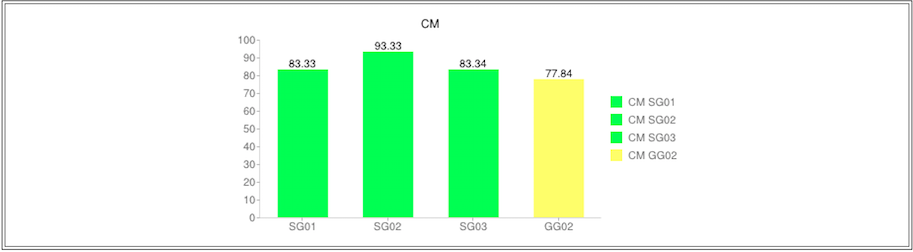
\includegraphics[width=0.7\textwidth]{ITmarkresults1}
		\caption{ITMark Appraisal tool result example}
		\label{fig:itmark_result1}
	\end{center}
\end{figure}

The overall assessment results will be available on a bar graph like the one presented in Figure \ref{fig:itmark_result2}, where we can see the maturity level associated.

\begin{figure}[H]
	\begin{center}
		\leavevmode
		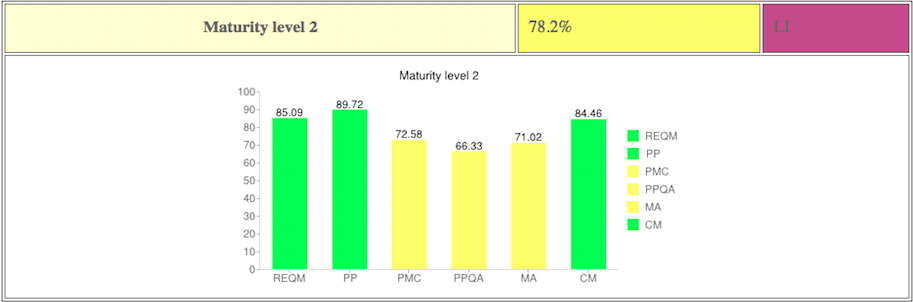
\includegraphics[width=0.7\textwidth]{ITmarkresults2}
		\caption{ITMark Appraisal tool result overall example}
		\label{fig:itmark_result2}
	\end{center}
\end{figure}

As will be explained in Section \ref{sec:question}, we take advantage of the questions in this tool to help in the assessment of the practices not evaluated automatically.